%% SECTION HEADER /////////////////////////////////////////////////////////////////////////////////////
\section{Displacements coupling at the interface of substructures}
\label{sec:interface}

%% SECTION CONTENT ////////////////////////////////////////////////////////////////////////////////////
The proposed model of the sandwich panel consisted of \ac{2d} and \ac{3d} elements.
In the combination of such elements, there are no common nodes because the nodes of the shell element are localised on the mid-plane of the component.
I realised the connection of both elements in a paper regarding the research on the effect of the glue thickness between the \ac{pzt} and the host plate on the propagation of elastic waves in a composite plate \cite{fiborek20192d}.
Connection was made possible by incorporating interface elements between both components.
The interface was implemented based on Lagrange multipliers, which are interpreted as forces imposed to determine the appropriate displacements of the nodes. My approach was similar to the interface for two shell elements proposed by Ashawin et al. \cite{ashwin2014formulation}.
To avoid creating coincided meshes for all components of \ac{hsc}, a non-matching interface should be used.
For this purpose, I proposed a novel approach for Lagrange multipliers-based interface, which creates a coupling matrix by the spectral elements shape function.
The non-matching interface was incorporated in the simulations of \ac{gw} registered by the \ac{fbg} optical sensor \cite{fiborek2022spectral}.
This paper is an original work regarding modelling such a sensor by the \ac{sem}.

\begin{figure}[!htb]
	\begin{center}
		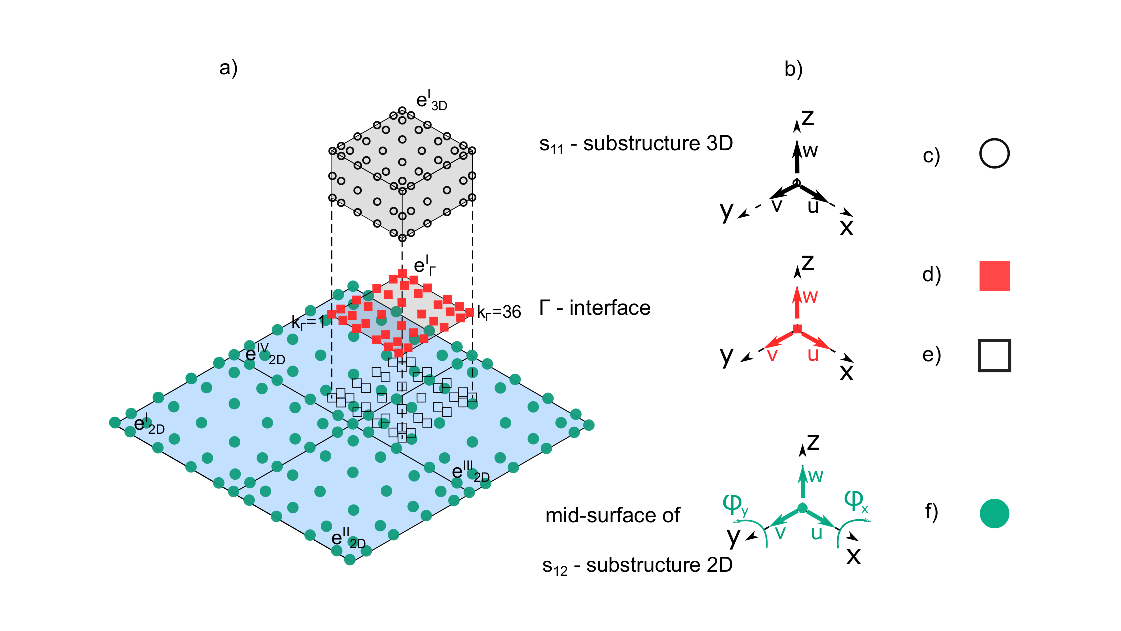
\includegraphics[width=1\textwidth]{Chapter_4/interface_2D3D}
	\end{center}
	\caption{Non-matching interface setup: (\textbf{a}) interface coupling, (\textbf{b}) the interface and the substructures degrees-of-freedom}
	\label{fig:interface}
\end{figure}
The non-matching interface between \ac{2d} and \ac{3d} elements is presented in Figure~\ref{fig:interface}.
The coupling of two domains imposes zero displacements relative to each other.
It can be expressed as
\begin{eqnarray}
	\left\{\begin{array}{c}
		\textbf{u}\\
		\textbf{v}\\
		\textbf{w}
	\end{array}\right\}_{s_{i1}}^{\Gamma^i}-
	\left\{\begin{array}{c}
		\textbf{u}\\
		\textbf{v}\\
		\textbf{w}
	\end{array}\right\}_{s_{i2}}^{\Gamma^i}=
	\left\{\begin{array}{c}
		\textbf{0}\\
		\textbf{0}\\
		\textbf{0}
	\end{array}\right\},
	\label{eq:coupling}
	\nomtypeD[Gamma]{$\Gamma$}{Interface}{}
\end{eqnarray}
where \(s_{i1}\) and \(s_{i2}\) are components connected by the interface \(\Gamma^i\).
For the whole structure, the Eq.~(\ref{eq:coupling}) can be written in the matrix form
\begin{eqnarray}
	\textbf{G}\textbf{d}=\textbf{0},
	\label{eq:cond_disp}
	\nomtypeD[G]{$\textbf{G}$}{Interface coupling matrix}{}
\end{eqnarray}
where \textbf{G} is the coupling matrix which contains the equations to interpolate the substructures displacements at the interfaces, and \(\textbf{d}\) is a global displacement field for \(nS\) number of substructures, composed as
\begin{eqnarray}
	\textbf{d} = \left\{\begin{array}{cccc}
		\textbf{d}_1, & \textbf{d}_2, &\ldots, & \textbf{d}_{nS}
	\end{array}\right\}^T.
	\label{eq:displacements}
\end{eqnarray}

\begin{algorithm}[!tbh]
	\SetAlgoLined
	\For{i = 1 \KwTo 2}{
		create \(n^{\Gamma}\times n^{s_i}\) null matrix 
		\(\mathbf{G}_i\),\\
		\For{j = 1 \KwTo \(n^{\Gamma}\)} {
			find \(ownerElement^j_i\) in the structure \(s_i\)
			containing interface node \(j\) with global coordinates vector: 
			\(X_p=(x^j_p,y^j_p)\)\;
			assign vector \(X_e=(x_e,y_e)\) of coordinates of all nodes in 
			\(ownerElement^j_i\)\;
			assign initial coordinates 
			\(X_{\kappa}=(x^j_{\kappa},y^j_{\kappa})\) to the nearest node in
			\(ownerElement^j_i\) to node \(j\)\;
			transform global coordinates \(X_{\kappa}\) to a local coordinate system \(\xi_{\kappa}=\xi(X_{\kappa}),\  
			\eta_{\kappa}=\eta(X_{\kappa})\)\;
			\While{\(\left|X_p-X_{\kappa}\right|>\mathrm{tol}\)}{
				\(\xi_{\kappa+1}=\xi_{\kappa}+(\mathcal{J}_{\kappa})^{1,1}_{\mathrm{inv}}(x^j_p-x_{\kappa}^j)
				+(\mathcal{J}_{\kappa})^{1,2}_{\mathrm{inv}}(y^j_p-y_{\kappa}^j)\)\,
				\(\eta_{\kappa+1}=\eta_{\kappa}+(\mathcal{J}_{\kappa})^{2,1}_{\mathrm{inv}}(x^j_p-x_{\kappa}^j)
				+(\mathcal{J}_{\kappa})^{2,2}_{\mathrm{inv}}(y^j_p-y_{\kappa}^j)\)\,
				\(X_{\kappa}=N_{\kappa+1}X_e\)\,
			}
			\(\mathbf{G}_i(j,n^{X_e})=N_{\kappa+1}\)\;
		}
		\uIf{\(s_i\) \(\mathrm{is\ 3D}\)} {
			\(\mathbf{G}_i=\left[\begin{array}{ccc}
				\mathbf{G}_i & \mathbf{0} & \mathbf{0}\\
				\mathbf{0} & \mathbf{G}_i & \mathbf{0}\\
				\mathbf{0} & \mathbf{0} & \mathbf{G}_i
			\end{array} \right]
			\)\;
		}
		\ElseIf{\(s_i\) \(\mathrm{is\ 2D}\)} {
			\(\mathbf{G}_i=\left[\begin{array}{ccccc}
				\mathbf{G}_i & \mathbf{0} & \mathbf{0} & 
				\frac{h_i}{2}\mathbf{G}_i & \mathbf{0}\\
				\mathbf{0} & \mathbf{G}_i & \mathbf{0} & \mathbf{0} & 
				\frac{h_i}{2}\mathbf{G}_i\\
				\mathbf{0} & \mathbf{0} & \mathbf{G}_i & \mathbf{0} & 
				\mathbf{0}
			\end{array} \right]\)\;
		}
	}
	\KwResult{coupling matrix \(\mathbf{G}=\left[\begin{array}{cc}
			\mathbf{G}_1 & \mathbf{G}_2
		\end{array} \right]\)}
	where \(s_i\) is one of the coupled structures,\;
	\(n^{\Gamma}\) and \(n^{s_i}\) are node numbers of the interface and node numbers of the structure \(s_i\), respectively \; \(\left(\mathcal{J}_{\kappa}\right)_{\mathrm{inv}}\) is the inverse Jacobian matrix evaluated at \((\xi_{\kappa},\eta_{\kappa})\)\;
	\(N_{\kappa+1}\) is the shape function evaluated at \((\xi_{\kappa+1},\eta_{\kappa+1})\)\;
	\(n^{X_e}\) is the vector of global order numbers of all nodes in the \(ownerElement^j_i\)\;
	\(h_i\) is a thickness of the structure \(s_i\) and tol is a termination criterion for iterations.
	\caption{Interface coupling matrix formulation}
	\label{alg:G_matrix}
	\nomtypeD[Jacobian]{$\mathcal{J}$}{Jacobian matrix}{}%
	\nomtypeD[nmn]{$n,m,n$}{Nodes numbers}{}%
	\nomtypeR[Xp]{$X_p$}{Coordinates vector of the interface point}{}{\unit{\metre}}%
	\nomtypeR[Xe]{$X_e$}{Coordinates vector of the element nodes}{}{\unit{\metre}}%
\end{algorithm}
General formulation of the matrix \textbf{G} is presented in Algorithm \ref{alg:G_matrix}.
The main task in this procedure was to calculate shape functions for each adjacent substructure at the points \(X_p=(x_p^k,y_p^k)\), which are projections of the interface nodes onto these substructures.
The shape function can be calculated after finding an owner element and local coordinates of the points.
Owner element is a spectral element in the domain of the substructure \(s_{ij}\) which contains interface node, for example, interface node \(k_\Gamma=36\) shown in~Figure~\ref{fig:interface}(\textbf{a}) is located in the element \(e^{I}_{3\mathrm{D}}\) and \(e^{III}_{2\mathrm{D}}\) for the substructures \(s_{11}\) and \(s_{12}\), respectively.
It can be found in two ways: using Matlab's built-in function \verb+inpolygon+ or more efficient procedure proposed by Silva et al. \cite{silva2009exact} which was used in the current implementation.
In this procedure, an initial approximation was first performed by rejecting all external points outside the rectangular region bounded by the points \(\mathrm{P_{min}}\) and \(\mathrm{P_{max}}\) as shown in Figure \ref{fig:b_b_test}(\textbf{a}).
If \(\mathrm{X_p}\) is inside the element, then the vectors \(\vec{V}_1\) and \(\vec{V}_2\) have the same direction.
\(\vec{V}_1\) and \(\vec{V}_2\) are defined as
\begin{eqnarray}
	\vec{V}_1 & = & \vec{v}_1\times \vec{v}_p,\\
	\vec{V}_2 & = & \vec{v}_p\times \vec{v}_2.
\label{eq:v_vectors}
\nomtypeD[vvv]{$\vec{v}_p,\,\vec{v}_1,\,\vec{v}_2$}{Cross-product test  vectors}{}%
\nomtypeD[V1]{$\vec{V_1}$}{First cross-product vector}{}%
\nomtypeD[V2]{$\vec{V_2}$}{Second cross-product vector}{}%
\end{eqnarray}
The vectors \(\vec{v}_p\), \(\vec{v_1}\) and \(\vec{v_2}\) are pictured in Figure \ref{fig:b_b_test}(\textbf{b}). \(\vec{V}_1\) and \(\vec{V}_2\) have the same direction if the inequality \(\vec{V}_1 \cdot \vec{V}_2 \geq0\) is satisfied for each element vertex.
Then, the transformation from global to local coordinates was realised by the iterative method presented in the work of Li et al.~\cite{li2014efficient} (see also \verb+while-loop+ in Algorithm~\ref{alg:G_matrix}).
\begin{figure}[!tbh]
	\begin{center}
		\includegraphics[width=0.95\textwidth]{Chapter_4/b_b_test}
	\end{center}
	\caption{Owner element for Xp interface node (\textbf{a}) boundary test, (\textbf{b}) cross-product test}
	\label{fig:b_b_test}
\end{figure}
As the cross product test is applicable only for elements with linear edges, in the case of boundaries approximated by second-order elements, this test was omitted.

The computational effectiveness of Algorithm~\ref{alg:G_matrix} can be easily improved if certain precautions are taken.
Firstly, the mesh of the interface has to be based on the mesh from one of the substructures \(s_{i}\), which may be referred to as a slave.
Shape functions evaluated at (\(\xi\), \(\eta\)) may take only zero and one values.
Moreover, the code was vectorised rather than using a for-loop form, provided that the required matrix of size \(4n^e\times n^{\Gamma}\), where \(n^e\) is the number of elements of the structure \(s_i\) elements, does not exceed the operating memory.